\documentclass[11pt,a4paper]{article}

\usepackage[margin=2cm, top=1.6cm, bottom=1.8cm]{geometry}
\usepackage{hyperref}
\usepackage{xcolor}
\usepackage{booktabs}
\usepackage{enumitem}
\usepackage{tabularx}
\usepackage{caption}
\usepackage{tikz}
\usetikzlibrary{arrows.meta, positioning}

\definecolor{darktext}{HTML}{1a1a1a}
\definecolor{graytext}{HTML}{555555}

\hypersetup{colorlinks=true, urlcolor=darktext, linkcolor=darktext}

\setcounter{secnumdepth}{0}
\pagenumbering{gobble}
\setlength{\parskip}{0.35em}
\setlength{\parindent}{0em}
\renewcommand{\baselinestretch}{1.05}

% tighter captions
\captionsetup{font=small, skip=3pt}

\begin{document}

% --- Title ---
\begin{center}
{\Large\bfseries CroissantMiner: Automated Croissant Metadata Extraction for ML Datasets}\\[0.7em]
{Berke Arda \quad Dr.\ Mubashara Akhtar}\\[0.2em]
{\small\color{graytext} ETH AI Center, ETH Zurich\quad\textbar\quad \href{mailto:bearda@student.ethz.ch}{bearda@student.ethz.ch}\quad\textbar\quad \href{https://github.com/berkearda/croissantminer}{github.com/berkearda/croissantminer}}
\end{center}

\vspace{0.1em}
\noindent\rule{\textwidth}{0.4pt}
\vspace{0.15em}

% --- Motivation ---
\textbf{Motivation.}\quad
RAI metadata fields in Croissant---data collection protocols, annotation demographics, biases, limitations---are almost entirely unpopulated across major dataset platforms, yet the NeurIPS Datasets \& Benchmarks track now requires Croissant metadata for all submissions. Platforms auto-generate basic fields, but RAI attributes must be filled manually. CroissantMiner automates this by extracting Croissant-compatible metadata from academic papers and dataset cards using LLMs.

\vspace{0.15em}

% --- Pipeline ---
\begin{center}
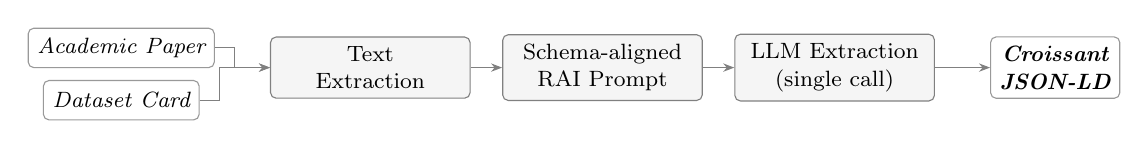
\begin{tikzpicture}[
    node distance=0.15cm and 0.4cm,
    block/.style={rectangle, rounded corners=2pt, draw=black!50, fill=black!4, minimum height=0.6cm, font=\footnotesize, align=center, text width=2.3cm},
    source/.style={rectangle, rounded corners=2pt, draw=black!40, minimum height=0.5cm, font=\footnotesize\itshape, align=center},
    arrow/.style={-{Stealth[length=4pt]}, black!50}
]
    \node[source] (paper) {Academic Paper};
    \node[source, below=0.15cm of paper] (card) {Dataset Card};
    \node[block, right=0.7cm of paper, yshift=-0.25cm] (extract) {Text\\Extraction};
    \node[block, right=of extract] (prompt) {Schema-aligned\\RAI Prompt};
    \node[block, right=of prompt] (llm) {LLM Extraction\\(single call)};
    \node[source, right=0.7cm of llm] (output) {\textbf{Croissant}\\\textbf{JSON-LD}};

    \draw[arrow] (paper.east) -- ++(0.25,0) |- (extract.west);
    \draw[arrow] (card.east) -- ++(0.25,0) |- (extract.west);
    \draw[arrow] (extract) -- (prompt);
    \draw[arrow] (prompt) -- (llm);
    \draw[arrow] (llm) -- (output);
\end{tikzpicture}
\end{center}

\vspace{0.1em}

% --- Approach ---
\textbf{Approach.}\quad
Given a PDF manuscript and its associated dataset card, CroissantMiner extracts the full document text and combines it with a carefully engineered prompt containing all 30 Croissant field definitions (10 general + 20 RAI) with extraction guidelines. The entire document is processed in a single LLM call (Claude Sonnet 4.5, 200K context), which produces a structured JSON-LD file aligned to the Croissant schema. This approach leverages the large context windows of modern LLMs to perform cross-section synthesis---the model sees the full paper and can connect information scattered across methodology, ethics, and appendix sections. A key insight is \textit{source complementarity}: dataset cards provide technical specifications (licensing, URLs, splits) while papers contribute methodological context and RAI information---combining both sources substantially improves extraction quality.

\vspace{0.1em}

\textbf{Evaluation (8 datasets, 30 fields).}\quad
Evaluated on 8 benchmark datasets (vision, NLP, speech, multimodal) across all 30 Croissant fields with \textbf{63.8\% average fill rate}. Claude Sonnet 4.5 achieves \textbf{70.6\% accuracy}, tied with Gemini 2.5 Pro and outperforming GPT-4o-mini (64.7\%). RAI fields reach \textbf{76.0\% accuracy} while general metadata reaches \textbf{67.3\%}---dedicated methodology and ethics sections in papers enable more reliable RAI extraction than scattered general metadata. Performance ranges from 84.4\% (Visual Genome) to 56.2\% (MMLU)---documentation quality remains the primary driver. Three fields achieve perfect extraction (name, URL, collection timeframe), while publication metadata (publisher, live dataset status) remains challenging.

\vspace{0.35em}

% --- Results Tables side by side ---
\begin{minipage}[t]{0.46\textwidth}
\centering
\captionof{table}{Model comparison (8 datasets, 30 fields).}
\small
\begin{tabular}{lc}
\toprule
\textbf{Method} & \textbf{Acc.} \\
\midrule
Claude Sonnet 4.5 & \textbf{70.6\%} \\
Gemini 2.5 Pro & \textbf{70.6\%} \\
GPT-4o-mini & 64.7\% \\
\bottomrule
\end{tabular}
\end{minipage}
\hfill
\begin{minipage}[t]{0.46\textwidth}
\centering
\captionof{table}{Field category performance.}
\small
\begin{tabular}{lcc}
\toprule
\textbf{Category} & \textbf{Fields} & \textbf{Acc.} \\
\midrule
General & 10 & 67.3\% \\
RAI & 20 & \textbf{76.0\%} \\
\midrule
Overall & 30 & 70.6\% \\
\bottomrule
\end{tabular}
\end{minipage}

\vspace{0.4em}

% --- Scale-up ---
\textbf{Ongoing: building the first large-scale Croissant metadata benchmark.}\quad
We have processed 103 datasets and are conducting a community annotation study across the full Croissant RAI vocabulary (30 fields: 10 general + 20 RAI). Annotators from the MLCommons Croissant community are validating extractions to establish the first comprehensive ground truth for automated metadata extraction at scale.

\vspace{0.15em}

% --- Integration ---
\textbf{Potential integration with the NeurIPS D\&B track.}
\vspace{0.05em}

\begin{tabularx}{\textwidth}{@{}lX@{}}
\textit{For authors:} & Upload a paper and receive a pre-filled Croissant file with RAI fields---review, correct, and submit alongside the manuscript. \\[0.2em]
\textit{For reviewers:} & Structured metadata summary highlighting documented vs.\ missing RAI fields, enabling targeted feedback. \\[0.2em]
\textit{With Eclair:} & CroissantMiner extracts from papers; Eclair handles dataset files---full metadata coverage.
\end{tabularx}

\vspace{0.3em}
\noindent\rule{\textwidth}{0.4pt}
\vspace{0.1em}
{\small\color{graytext} Built on the Croissant metadata format (Akhtar et al., NeurIPS 2024 Spotlight). Paper in preparation. \hfill February 2026}

\end{document}
